\documentclass[11pt,oneside]{article}



\usepackage{inputenc}
\usepackage[english,russian]{babel} % Windows
%\usepackage{vestnik}
\usepackage{cite}
\usepackage{fixltx2e}
\usepackage{multirow} % Слияние строк в таблице

\usepackage{graphicx} % Вставляю рисунки
\graphicspath{{D:/latex-tasks/lab-6/images}{images/}} % Папка с картинками
\setlength\fboxsep{3pt} % Отступ рамки \fbox{} от рисунка
\setlength\fboxrule{1pt} % Толщина линий рамки fbox{}

\setcounter{page}{1}

\usepackage[pdftex, unicode, bookmarks, pagebackref]{hyperref}

\begin{document}

	\newcommand{\phan}{\hspace*{0cm}}
	\newcommand{\comment}{}

	\author{А.В. Автор}
	\title{МОДЕЛЬ ВАРИАНТОВ ИСПОЛЬЗОВАНИЯ ПАРАЛЛЕЛЬНОЙ СИСТЕМЫ УПРАВЛЕНИЯ БАЗАМИ ДАННЫХ ДЛЯ ГРИД}
	\maketitle{}

	% оформление аннотации
	\begin{abstract}
		Работа посвящена вопросам проектирования параллельных систем управления базами данных для грид-систем. Описан механизм параллельной обработки запросов и проблема появления перекосов. Описана модель вариантов использования системы. Приведено описание ключевых подсистем, даны спецификации и диаграммы вариантов использования данных подсистем.
	\end{abstract}


	\markboth{А.В. Автор}{Модель вариантов использования ПСУБД}
	
	\section*{Введение}
	\par В связи со значительным ростом хранимой в электронном виде информации системы баз данных используются для управления петабайтами данных. Типичным примером сверхбольших баз данных являются научные базы данных, накапливающие информацию, поставляемую ускорителями элементарных частиц. Такие базы данных могут эффективно поддерживаться и обрабатываться параллельными системами управления базами данных (ПСУБД).
	\par По этой причине в настоящее время одним из перспективных направлений в области параллельных систем баз данных является разработка систем управления базами данных для грид-систем. В такой системе процессорные устройства, память, диски и проч. связываются друг с другом в соответствии с некоторой иерархией. На первом уровне иерархии находятся процессорные ядра, размещенные на одном кристалле. На втором уровне находятся многоядерные процессоры, объединенные в многопроцессорные модули общей памятью (SMP). На третьем уровне SMP-модули объединяются в кластер с помощью высокоскоростной соединительной сети. Четвертый уровень представляют грид-системы, включающие в себя несколько кластеров. Корпоративные грид-системы могут объединяться в кооперативные грид-объединения на базе Интернет. И так далее.
	\par Параллельным системам управления базами данных посвящено большое количество работ~\cite{B_Gray2005, B_Mehta1997, B_Williams1998}. Однако проблематика систем баз данных с иерархической архитектурой исследована мало. Сравнительный анализ архитектур параллельных систем баз данных показан в табл. ~\ref{Tab:t}

	\begin{table}[h!]
		\begin{tabular}{|l|c|c|c|c|c|c|}
			\hline
			& \textit{\textbf{SE}} & \textbf{S} & \textbf{SN} & \textbf{CE} & \textbf{CD} & \textbf{C}$_D$ \\
			& & \textbf{D} & & & & \\
			\hline
			\textbf{Масштабируемость} & $0$ & $1$ & $2$ & $3$ & $3$ & $3$ \\
			\hline
			\textbf{Доступность данных} & $0$ & $1$ & $3$ & $1$ & $2$ & $2$ \\
			\hline
			\textbf{Баланс загрузки} & $3$ & $2$ & $0$ & $2$ & $1$ & $1$ \\
			\hline
			\textbf{Межпроцессорные коммуникации} & \multirow{2}{*}{$3$} & \multirow{2}{*}{$0$} & \multirow{2}{*}{$0$} & \multirow{2}{*}{$2$} & \multirow{2}{*}{$1$} & \multirow{2}{*}{$1$} \\
			& & & & & & \\
			\hline
			\textbf{Когерентность кэшей} & $2$ & $0$ & $3$ & $2$ & $0$ & $3$ \\
			\hline
			\textbf{Организация блокировок} & $2$ & $0$ & $3$ & $2$ & $0$ & $3$ \\
			\hline
			\textit{\textbf{Сумма баллов}} & $10$ & $4$ & $11$ & $12$ & $7$ & $13$ \\
			\hline
		\end{tabular}
		\label{Tab:t}
	\end{table}
	
	\par Целью настоящей статьи является описание спецификации ПСУБД для грид-систем, разрабатываемой в рамках проекта "<Омега">\cite{B_OMEGA}. Спецификация параллельной СУБД для грид разработана с учетом распределенного характера системы, неоднородности вычислительных узлов и соединительной сети. ПСУБД проектируется таким образом, чтобы изолировать пользователя от сложной структуры и технологий, лежащих в основе грид-системы. Требования к ПСУБД задаются при помощи модели вариантов использования, построенной на основе языка моделирования UML версии 2.0.
	\par Оставшаяся часть статьи организована следующим образом. В разделе~\ref{S_ParQueryProcessing} описана общая схема обработки запроса в ПСУБД. В разделе ~\ref{S_UseCaseModel} приведено модели вариантов использования, приведено описание структуры ПСУБД, форматы входных и выходных данных, диаграммы вариантов использования и описание вариантов использования. В заключении суммируются основные результаты и описаны направления дальнейшей работы.
	
	\section{Организация параллельной обработки запросов}\label{S_ParQueryProcessing}
	\par Вопросам организации параллельной обработки запросов в многопроцессорных системах посвящен целый ряд работ (см. например~\cite{B_Sokolinsky2001, B_Aloisio2005, B_Dutra2004}). Одной из основных форм параллельной обработки запросов является \textit{фрагментный параллелизм}. Фрагментный параллелизм предполагает \textit{фрагментацию} \---~разбиение на непересекающиеся части каждого отношения базы данных. Фрагменты отношения распределяются по различным процессорным узлам многопроцессорной системы. Основная идея заключается в том, чтобы преобразовать запрос в набор параллельных агентов, каждый из которых будет обрабатывать свою часть запроса на выделенном для него процессорном узле. При этом он будет использовать расположенный на данном узле фрагмент и (возможно) результаты работы других агентов. В работе~\cite{B_Sokolinsky2001}~преобразование запроса в набор параллельных агентов достигается путем вставки специального оператора \texttt{exchange}~в дерево запроса. Схема обработки запроса в таком случае будет выглядеть следующим образом (рис. ~\ref{fig:qexec}).
	
	\begin{figure}[h]
		\centering
		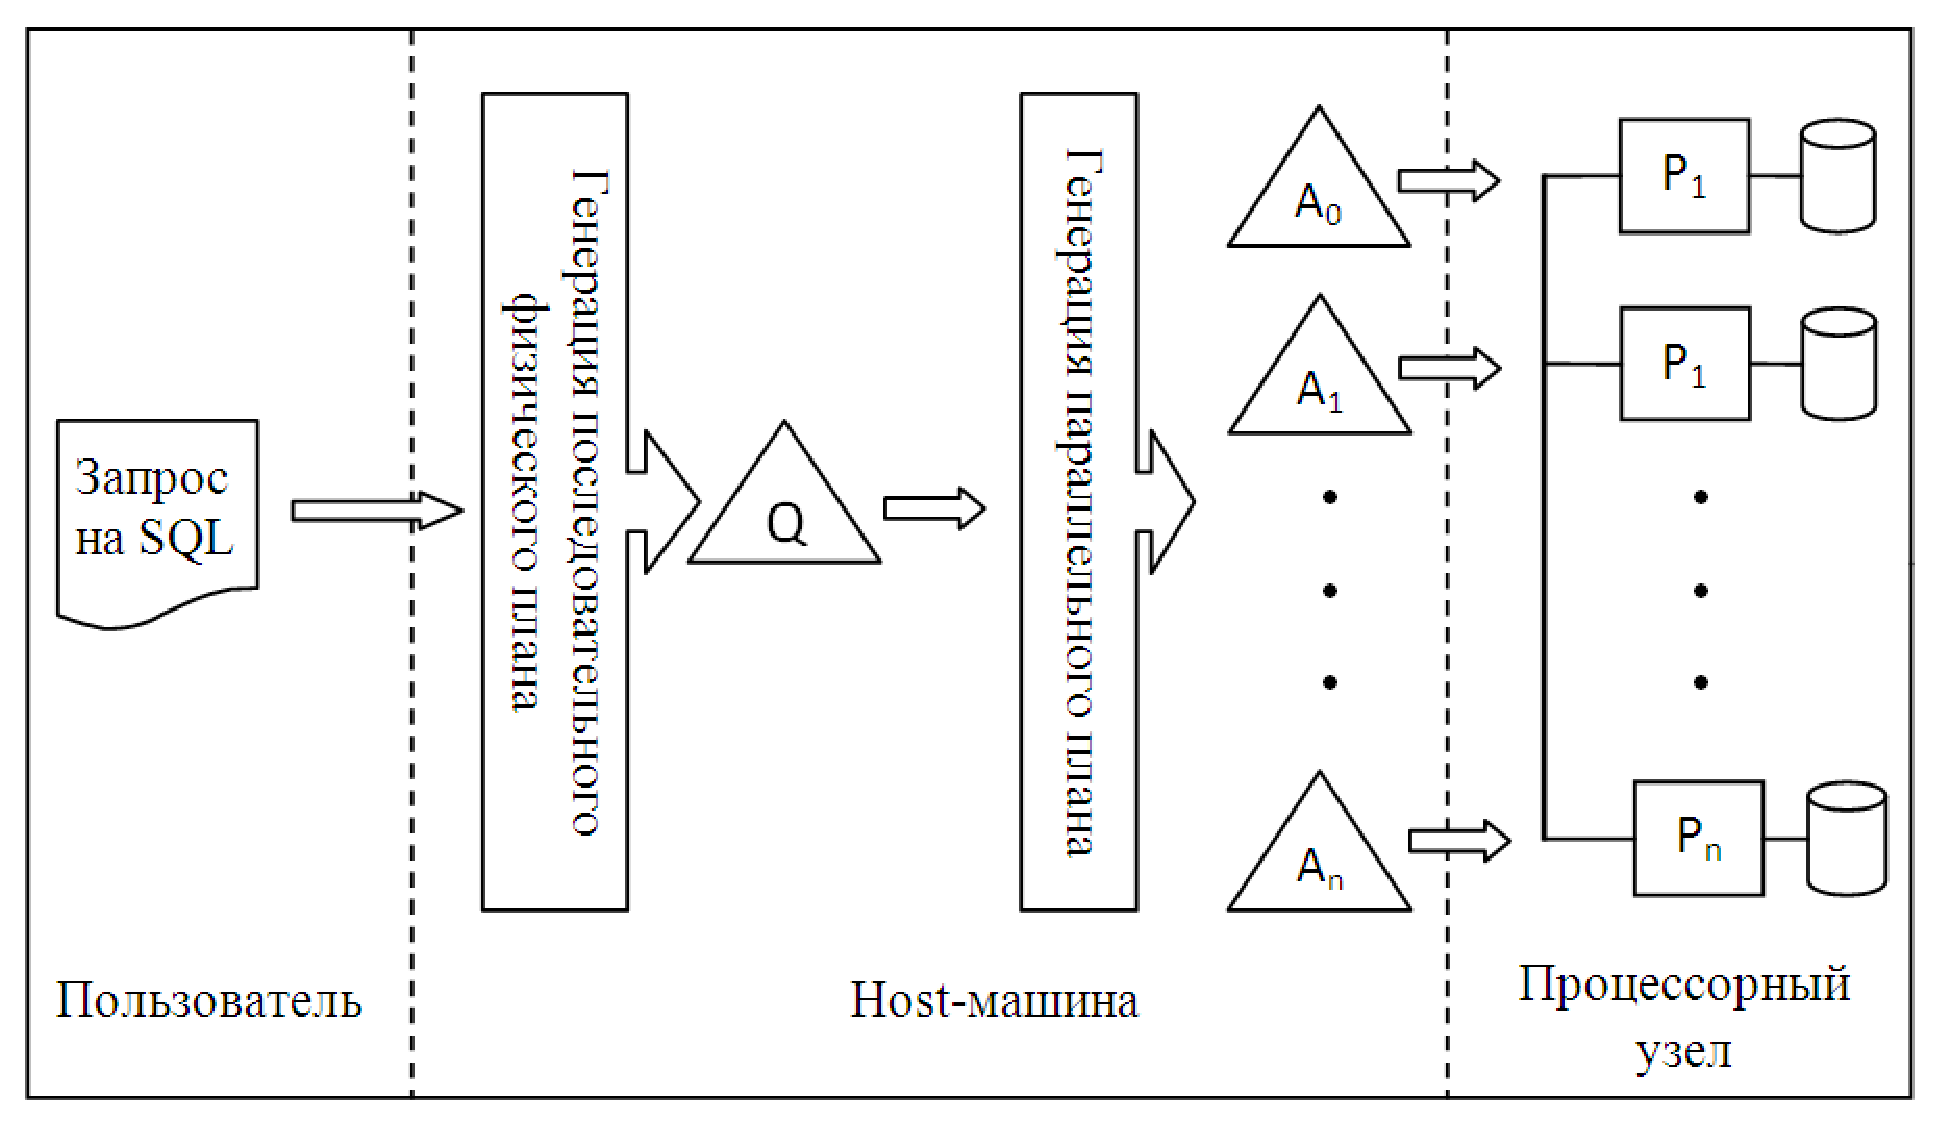
\includegraphics[width=0.7\linewidth]{qexec}
		\caption{}
		\label{fig:qexec}
	\end{figure}	
	
	\par Пусть система имеет состоит из $n$ процессорных узлов. В соответствии со схемой, представленной на рис.~\ref{fig:qexec} запрос на языке SQL передается пользователем на host-машину, где он транслируется в некоторый \textit{последовательный физический план}. Данный физический план преобразуется в \textit{параллельный план}, представляющий собой совокупность параллельных агентов. Это достигается путем вставки параллельного оператора \texttt{exchange} в соответствующие места дерева запроса. Оператор \texttt{exchange} организует взаимодействие параллельных агентов и обеспечивает пересылку кортежей между агентами в тех случаях, когда это необходимо.
	\par На следующем этапе параллельные агенты пересылаются c host-машины на соответствующие процессорные узлы, где \textit{интерпретируются} исполнителем запросов. Результаты выполнения агентов объединяются корневым оператором \texttt{exchange} на выделенном процессорном узле.
	\par Большое негативное влияние на производительность параллельных СУБД для многопроцессорных систем оказывает проблема перекосов. Суть проблемы заключается в следующем. При параллельной обработке запроса каждый агент обрабатывает свою часть запроса на отдельном процессорном узле. В этом случае возникает ситуация, когда один или несколько агентов завершают обработку, в то время как остальные (загруженные) агенты активно работают. Таким образом, при обработке запроса часть процессорных узлов может простаивать, что уменьшает эффект от распараллеливания и увеличивает время обработки запроса. Подобные ситуации могут возникать вследствие неоднородности процессорных узлов, при неравномерном распределении базы данных по процессорным узлам и т.д.
	\par Одним из наиболее известных способов решения данной проблемы является использование алгоритмов балансировки загрузки, основанных на репликации базы данных. В работе~\cite{B_Lepikhov2006} в качестве стратегии репликации предлагается метод частичного зеркалирования. При использовании данной стратегии каждый фрагмент на логическом уровне разбивается на равномощные сегменты, являющиеся единицами репликации данных и балансировки загрузки. Фрагмент, расположенный на одном узле частично реплицируется на остальных узлах многопроцессорной системы. Размер реплицируемой части фрагмента на каждом узле задается некоторым коэффициентом репликации. 
	\par Общую схему алгоритма балансировки загрузки с использованием метода частичного зеркалирования можно описать следующим образом. При возникновении ситуации перекоса агент, выполнивший свою часть запроса (простаивающий), переходит в состояние простоя и выбирает наиболее загруженного агента. Загруженный агент получает от простаивающего агента предложение передать часть работы. Загруженный агент оценивает состояние обработки запроса и выделяет часть своего фрагмента  простаивающеиу агенту. При этом, если на узле простаивающего агента имеется реплика этого фрагмента, то пересылки по сети не требуются: простаивающий агент переходит в состояние выполнения и использует для обработки реплику фрагмента, используемого загруженным агентом. Таким образом уменьшаются накладные расходы на передачу данных по сети, уменьшается время, затрачиваемое системой на операцию балансировки загрузки.
	\par Подобные методы позволяют уменьшить негативный эффект ситуации перекоса: уменьшить время простоя процессорного узла и время обработки запроса.
	
	\section{Модель вариантов использования}\label{S_UseCaseModel}
	\par Модель вариантов использования предоставляет возможность описать требования в наглядной и удобной для разработчика форме с акцентом на значимость получаемых результатов для каждого пользователя или внешней системы. Она предоставляет исходные данные для процессов реализации и тестирования программного продукта. Модель вариантов использования состоит из актеров, вариантов использования и связей между ними. Актер представляет собой пользователя системы или внешнюю подсистему, взаимодействующую с разрабатываемой системой. Вариант использования представляет собой последовательность действий, которую система должна выполнять, взаимодействуя с актерами. Для удобства разработчика, модель вариантов использования представляется в виде диаграмм, на которых отображаются варианты использования и взаимодействующие с ними актеры.
	\par В данной работе вариант использования  описывается в соответствии со следующей дисциплиной. Во-первых, приводится краткое описание варианта использования и предварительные условия, необходимые для начала его выполнения. Во-вторых, приводится описание основных шагов, составляющих поток событий варианта использования. В-третьих, обсуждаются альтернативные потоки событий, приводятся дополнительные требования.
	\par Данный раздел статьи организован следующим образом. В подразделе~\ref{S_PDBMSRequirements} описываются требования к ПСУБД, В подразделе~\ref{S_InOutData} описан формат запроса и формат результата. Подраздел~\ref{S_PDBMSStructure} посвящен описанию стуруктуры ПСУБД. Далее до конца главы описываются подсистемы ПСУБД и варианты их использования.
	
	\subsection{Общие требования к ПСУБД}\label{S_PDBMSRequirements}
	\par Параллельная система управления базами данных (ПСУБД) представляет собой программную систему, которая предназначена для параллельной обработки запросов в иерархических мультипроцессорных системах.
	
	\par ПСУБД поддерживает фрагментный параллелизм и имеет механизм балансировки загрузки, основанный на стратегии репликации, называемый методом частичного зеркалирования~\cite{B_Lepikhov2006}. Заложенный в ПСУБД параллелизм обработки запросов прозрачен для пользователя.
	
	\par ПСУБД поддерживает многопользовательский режим работы, т.е. одновременно система может обрабатывать запросы нескольких пользователей.
	Для организации приема запросов от пользователей в ПСУБД использован реляционный язык запросов RQL (см. раздел~\ref{S_RQL}). Запрос, записанный на языке RQL, передается ПСУБД в виде текстового файла. После окончания обработки запроса ПСУБД передает пользователю \textit{результирующую таблицу} и \textit{лог-файл}.
	
	\par Результирующая таблица представляется в виде текстового файла в формате CSV (Comma Separated Value)~\cite{B_RFC4180}. Если результатом запроса является пустая таблица, то текстовый файл с результирующей таблицей будет пустым.
	\par Лог-файл передается пользователю в виде текстового файла в формате CSV. Лог-файл содержит диагностические сообщения о ходе выполнения запроса. Структура и семантика сообщений лог-файла определены в разделе~\ref{S_LOG}.
	
	\subsection{Формат входных и выходных данных}\label{S_InOutData}
	\subsubsection{Спецификация языка RQL}\label{S_RQL}
	\par Язык запросов RQL (Relational Query Language) базируется на реляционной алгебре. Описанная здесь нотация включает в себя операции простой выборки и эквисоединения. Простая выборка (\texttt{Restrict}) допускает только условия следующего вида: \texttt{<Атрибут> <Операция сравнения> <Константа>}. Операция эквисоединения (\texttt{eQuijoin}) выполняет соединение по равенству одной пары атрибутов. Предложенная нотация может быть легко распространена на другие реляционные операции.
	\par В качестве разделителя лексем могут использоваться пробелы, символы табуляции, перевода строки и возврата каретки в любом количестве и сочетании.
	\par Грамматика языка RQL, описанная с помощью нотации Бэкуса-Наура представлена ниже:\\
	\texttt{<Запрос> ::= <Оператор>\\
		<Запрос> ::= <Запрос>;<Оператор>\\
		<Оператор> ::= <Метка> <Реляционная операция>\\
		<Реляционная операция> ::= <Выборка> | <Эквисоединение>\\
		<Выборка> ::= R <Условие> <Таблица>\\
		<Условие>::= <Номер атрибута> <Операция сравнения> <Константа>\\
		<Эквисоединение> ::= Q <Номер атрибута> <Номер атрибута> <Таблица> <Таблица>\\
		<Таблица> ::= <Метка> | <Идентификатор хранимой таблицы>\\
		<Метка> ::= <Целое без знака>\\
		<Номер атрибута> ::= <Целое без знака>\\
		<Операция сравнения> ::= > | < | = <Идентификатор хранимой таблицы> ::= \#<Целое без знака>
	}
	
	\subsubsection{Спецификация лог-файла}\label{S_LOG}
	Лог-файл содержит диагностические сообщения, выдаваемые ядрами ПСУБД.
	В качестве разделителя лексем могут использоваться пробелы, символы табуляции, перевода строки и возврата каретки в любом количестве и сочетании. Описание структуры лог-файла в нотации Бэкуса-Наура представлена ниже:\\
	\texttt{<Лог-файл> ::= <Сообщение>\{<Сообщение>\}\\
		<Сообщение> ::= <Ядро> <Результат> <Комментарий>\\
		<Ядро> ::= <Целое без знака>\\
		<Результат> ::= <Целое без знака>\\
		<Комментарий> ::= <Строка>
	}
	
	\subsection{Структура ПСУБД}\label{S_PDBMSStructure}
	ПСУБД включает в себя три подсистемы: \textit{Клиент}, \textit{Координатор} и \textit{Ядро ПСУБД}. Клиент запускается на рабочей станции пользователя и обслуживает только этого пользователя. В многопроцессорной системе, среди выделенных для ПСУБД процессорных узлов, выделяется специальный узел, на котором размещается Координатор. На каждом не занятом Координатором процессорном узле запускается экземпляр Ядра ПСУБД (на отдельном узле размещается одно Ядро ПСУБД).
	\par Общая схема взаимодействия подсистем ПСУБД для случая трех пользователей и двух Ядер ПСУБД представлена на рис. ~\ref{fig:sysobjectdiagram}. 
	Размещение подсистем для этого случая показано на рис. ~\ref{fig:sysdeploydiagram}.
	
	\begin{figure}[h]
		\centering
		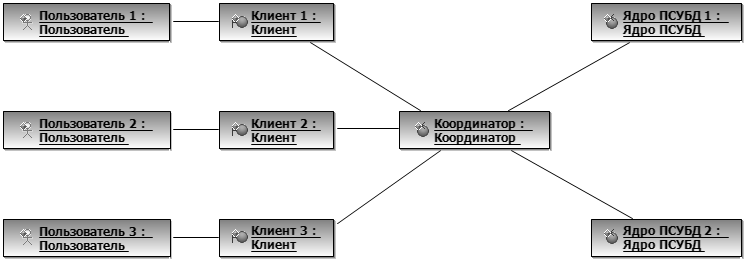
\includegraphics[width=0.9\linewidth]{sysobjectdiagram}
		\caption{}
		\label{fig:sysobjectdiagram}
	\end{figure}
	
	\begin{figure}[h]
		\centering
		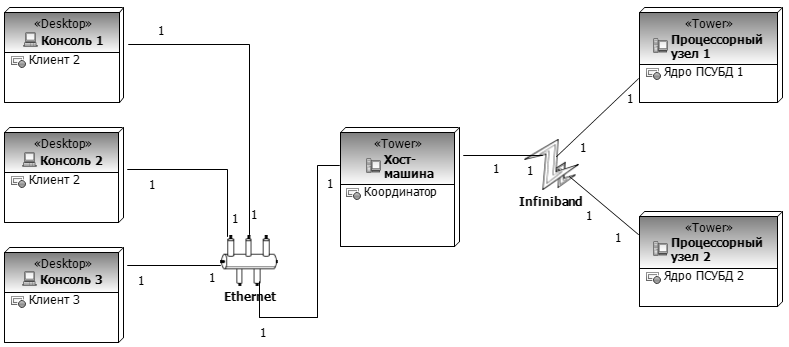
\includegraphics[width=0.9\linewidth]{sysdeploydiagram}
		\caption{}
		\label{fig:sysdeploydiagram}
	\end{figure}
	
	\subsection{Подсистема "<Клиент">}\label{S_Client}
	\par Клиент предоставляет пользователю интерфейс доступа к ПСУБД: обеспечивает передачу запросов ПСУБД, мониторинг процесса обработки запроса и доступ к результату его выполнения. Клиент может использоваться в диалоговом и пакетном режимах. При использовании Клиента в диалоговом режиме пользователю предоставляется диалоговое окно, основными элементами которого являются строка ввода запроса, область просмотра результата и область просмотра диагностических сообщений. При использовании Клиента в пакетном режиме Пользователь запускает его в командной строке. В качестве параметра Клиенту передается имя файла с запросом и имя файла, в который будет записана результирующая таблица.
	
	\subsection{Варианты использования подсистемы "<Клиент">}\label{S_ClientUseCase}
	
	\begin{figure}[h]
		\centering
		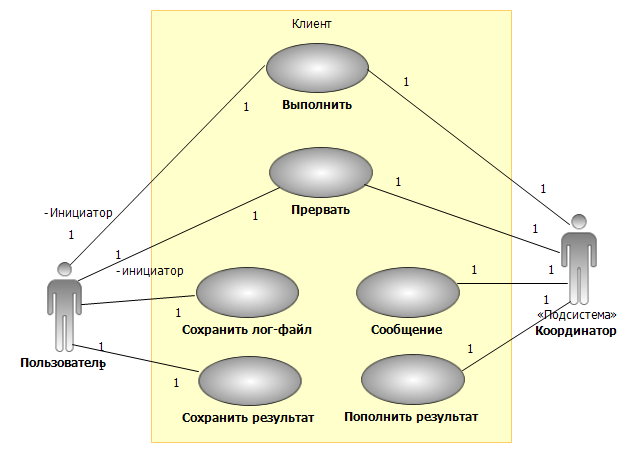
\includegraphics[width=0.9\linewidth]{clientUCDiagram}
		\caption{}
		\label{fig:clientucdiagram}
	\end{figure}
	
	
	Для подсистемы "<Клиент"> нами выделяются следующие варианты использования, приведенные на рис. ~\ref{fig:clientucdiagram}.
	: \textit{"<Выполнить">}, \textit{"<Прервать">}, \textit{"<Сообщение">}, \textit{"<Пополнить результат">}, \textit{"<Сохранить результат">}, \textit{"<Сохранить лог-файл">}. Варианты использования предусматривают диалоговый и пакетный режимы работы Клиента. Далее в этом разделе приводится детальное описание каждого варианта использования.
	
	\subsubsection{Вариант использования "<Выполнить">}
	Данный вариант использования передает запрос от Пользователя к Координатору. Вариант использования начинается, когда Пользователь указывает путь к текстовому файлу с запросом и активирует функцию "<Выполнить">. При этом Клиент должен находиться в состоянии ожидания запроса и текстовый файл с запросом должен существовать на узле Клиента.
	\par Поток событий состоит из следующей последовательности шагов. На первом шаге Клиент переходит в состояние выполнения запроса и подготавливает систему к обработке запроса: очищает область просмотра результирующей таблицы, очищает область просмотра сообщений, формирует пустой файл результата и пустой лог-файл. На втором шаге Клиент передает текстовый файл с запросом Координатору. Вариант использования завершается.
	\par Вариант использования предусматривает один альтернативный поток событий. Он начинает работу, если попытка Клиента передать запрос Координатору завершается неудачей. В этом случае Клиент выводит в области просмотра соответствующее сообщение об ошибке, записывает данное сообщение об ошибке в лог-файл и переходит в состояние ожидания нового запроса. Вариант использования завершается.
	
	\subsubsection{Вариант использования "<Прервать">}
	Данный вариант использования осуществляет прерывание выполнения (досрочное завершение) запроса по требованию Пользователя. Данный вариант использования начинается, когда Пользователь вызывает функцию "<Прервать">. При этом Клиент должен находиться в состоянии выполнения запроса.
	\par Поток событий состоит из следующей последовательности шагов. На первом шаге Клиент переходит в состояние вывода сообщения и посылает Координатору сообщение "<Прервать">. Если передача сообщения завершается успешно, то на втором шаге Клиент формирует сообщение о досрочном прерывании запроса, выводит его в области просмотра сообщений и записывает в лог-файл. на последнем шаге Клиент переходит в состояние ожидания нового запроса. Вариант использования завершается.
	\par Если попытка Клиента передать сообщение Координатору завершается неудачей, то он формирует сообщение об ошибке, выводит его в области просмотра и записывает в лог-файл. После этого Клиент переходит в состояние выполнения запроса. Вариант использования завершается.
	
	\subsubsection{Вариант использования "<Сообщение">}
	Данный вариант использования выполняет уведомление Клиента о возникновении некоторого существенного события в ходе выполнения запроса. Данный вариант использования начинается, когда Координатор вызывает функцию "<Сообщение">. При этом Клиент должен находиться в состоянии выполнения запроса.
	\par Поток событий состоит из следующей последовательности шагов. На первом шаге Клиент переходит в состояние вывода сообщения и получает от Координатора диагностическое сообщение. На втором шаге Клиент выводит полученное сообщение в области просмотра сообщений и записывает его в лог-файл. На третьем шаге Клиент переходит в состояние выполнения запроса. Вариант использования завершается.
	\par Вариант использования предусматривает следующий альтернативный поток событий. Он начинается, если Клиент на первом шаге получает от Координатора сообщение с кодом фатальной ошибки или кодом, соответствующим нормальному завершению. Альтернативный поток включает в себя следующую последовательность шагов. На первом шаге Клиент выводит полученное сообщение в области просмотра сообщений и записывает его в лог-файл. На втором шаге Клиент переходит в состояние ожидания нового запроса после чего вариант использования завершается.
	
	\subsubsection{Вариант использования "<Пополнить результат">}
	Данный вариант использования передает очередную часть результирующей таблицы от Координатора Клиенту. Вариант использования начинается, когда Координатор вызывает функцию "<Пополнить результат">.
	\par Поток событий состоит из следующей последовательности шагов. На первом шаге Клиент переходит в состояние вывода результата и принимает от Координатора очередную часть результирующей таблицы. На втором шаге Клиент выводит полученную часть результирующей таблицы в области просмотра результата и записывает ее в результирующий файл. На третьем шаге Клиент переходит в состояние выполнения запроса. Вариант использования завершается.
	
	\subsubsection{Вариант использования "<Сохранить результат">}
	Данный вариант использования cохраняет результат запроса в текстовом файле в формате CSV. Вариант использования начинается, когда Пользователь вызывает функцию "<Сохранить результат">. При этом Клиент должен находиться в состоянии ожидания нового запроса.
	\par Поток событий состоит из следующей последовательности шагов. На первом шаге Клиент переходит в состояние сохранения результата, запрашивает у Пользователя путь и имя файла для сохранения результирующей таблицы. На втором шаге Клиент сохраняет результирующую таблицу в текстовом файле, указанном пользователем, в формате~CSV. На третьем шаге Клиент переходит в состояние ожидания нового запроса. Вариант использования завершается.
	\par Полученная Клиентом результирующая таблица хранится во временном файле до тех пор, пока Пользователь не запустит выполнение нового запроса.
	
	\subsubsection{Вариант использования "<Сохранить лог-файл">}
	Данный вариант использования сохраняет результат запроса в текстовом файле в формате~CSV. Вариант использования начинается, когда Пользователь вызывает функцию "<Сохранить лог-файл">. При этом Клиент должен находиться в состоянии ожидания нового запроса.
	\par Поток событий состоит из следующей последовательности шагов. На первом шаге Клиент переходит в состояние сохранения лог-файла, запрашивает у Пользователя путь и имя файла для сохранения лог-файла. На втором шаге Клиент сохраняет лог-файл в текстовом файле, указанном пользователем. На третьем шаге Клиент переходит в состояние ожидания нового запроса. Вариант использования завершается.
	\par Вариант использования специфицирует следующее специальное требование: полученные Клиентом от Координатора сообщения хранятся во временном файле до тех пор, пока Пользователь не запустит выполнение нового запроса.
	
	\subsection{Подсистема "<Координатор">}\label{S_Coordinator}
	\par Координатор организует параллельное выполнение запроса. Координатор принимает запрос, поступающий от Клиента и рассылает его на некоторое множество Ядер ПСУБД. По завершении обработки запроса Координатор собирает поступающие от Ядер ПСУБД результаты и передает Клиенту.
	\subsection{Варианты использования подсистемы "<Координатор">}\label{S_CoordinatorUseCases}
	
	\begin{figure}[h]
		\centering
		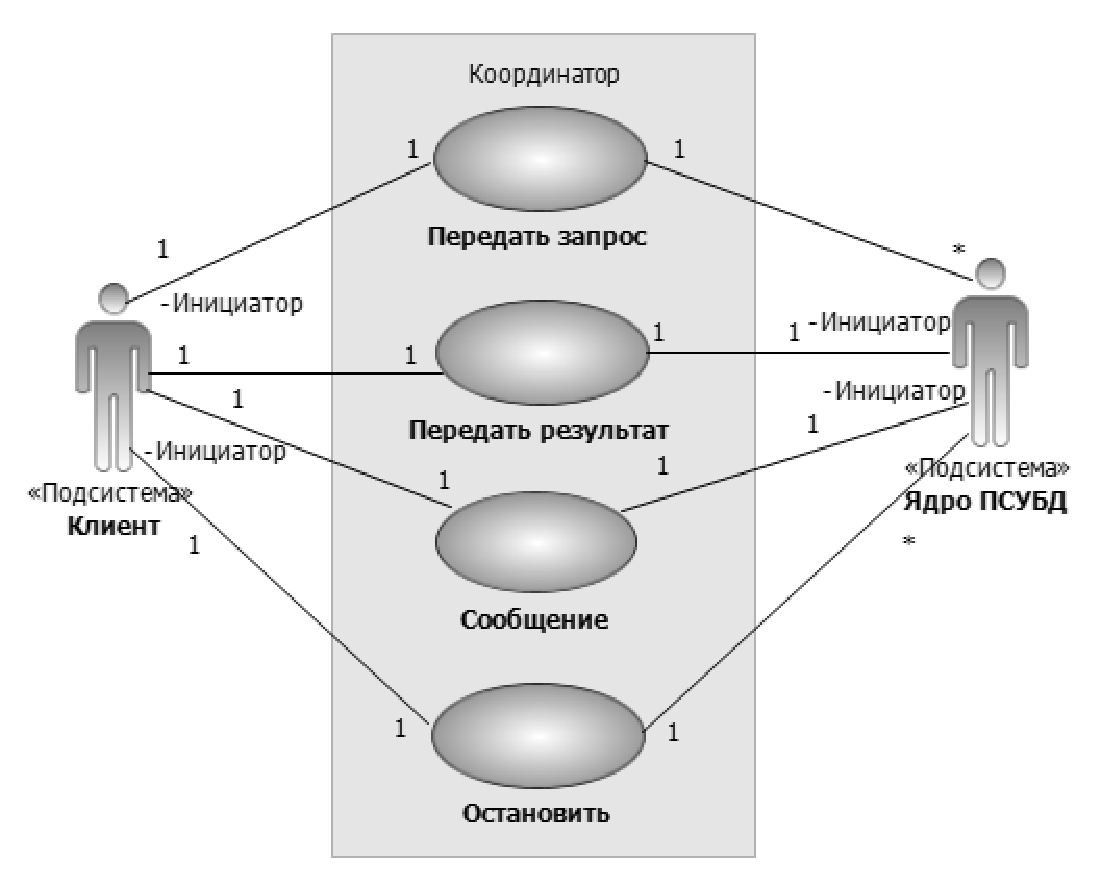
\includegraphics[width=0.9\linewidth]{coordUCDiagram}
		\caption{}
		\label{fig:coordUCDiagram}
	\end{figure}
	
	Для подсистемы "<Координатор"> нами были разработаны следующие варианты использования, приведенные на рис. ~\ref{fig:coordUCDiagram}.
	: \textit{"<Передать запрос">}, \textit{"<Передать результат">}, \textit{"<Сообщение">}, \textit{"<Остановить">}. Координатор взаимодействует с множеством Клиентов и должен представлять собой систему высокой готовности. Варианты использования спроектированы таким образом, чтобы максимально уменьшить время отклика Координатора. Далее в этом разделе приводится детальное описание каждого варианта использования.
	
	\subsubsection{Вариант использования "<Передать запрос">}
	\par Передает запрос Ядрам ПСУБД для дальнейшей обработки. Вариант использования начинается, когда Клиент вызывает функцию "<Передать запрос">.
	\par Поток событий состоит из следующей последовательности шагов. На первом шаге Координатор получает запрос от Клиента. На втором шаге Координатор подготавливает параллельную обработку запроса. На основе анализа файла конфигурации ПСУБД Координатор формирует список Ядер ПСУБД, которые будут участвовать в обработке запроса. На втором шаге Координатор формирует пустой файл результата и лог-файл. На третьем шаге Координатор передает запрос Ядрам ПСУБД в асинхронном режиме. Вариант использования завершается.
	
	\subsubsection{Вариант использования "<Передать результат">}
	\par Передает результирующую таблицу, выдаваемую Ядром ПСУБД, Клиенту. Вариант использования начинается, когда Ядро ПСУБД вызывает функцию "<Передать результат">.
	\par Поток событий состоит из следующей последовательности шагов. На первом шаге Координатор получает результат запроса в виде текстового файла от Ядра ПСУБД в синхронном режиме. На втором шаге Координатор анализирует полученный результат и формирует результирующую таблицу. На третьем шаге Координатор передает результирующую таблицу Клиенту. Вариант использования завершается.
	\par Если на первом шаге Координатор обнаруживает, что результирующая таблица получена от последнего задействованного в обработке запроса ядра ПСУБД, Координатор устанавливает флаг "<Запрос обработан">.
	\par Вариант использования включает в себя следующие два альтернативных потока.
	\par Если Координатору на третьем шаге основного потока событий не удается передать результирующую таблицу Клиенту, то начинается выполнение альтернативного потока, состоящего из следующих шагов. На первом шаге Координатор формирует системный лог-файл, предназначенный для вывода внутренних служебных сообщений Координатора и записывает в него сообщение "<Клиент недоступен">. На втором шаге Координатор устанавливает флаг "<Запрос обработан">. Вариант использования завершается.
	\par Если при выполнении основного потока событий на втором шаге Координатор обнаруживает, что установлен флаг "<Запрос обработан">, то он удаляет результирующую таблицу и завершает выполнение варианта использования.
	
	\subsubsection{Вариант использования "<Сообщение">}
	\par Уведомляет Координатор о возникновении некоторого существенного события, произошедшего с Ядром ПСУБД. Вариант использования начинается, когда Ядро ПСУБД вызывает функцию "<Сообщение">.
	\par Основной поток событий состоит из следующей последовательности шагов. На первом шаге Координатор получает лог-файл от Ядра ПСУБД. На втором шаге Координатор интерпретирует полученный лог-файл и формирует диагностическое сообщение для клиента. На последнем шаге Координатор передает данное сообщение Клиенту. Вариант использования завершается.
	\par Вариант использования включает в себя следующие два альтернативных потока.
	\par Если Координатору на третьем шаге основного потока событий не удается передать диагностическое сообщение Клиенту, то начинается выполнение альтернативного потока, состоящего из следующих шагов. На первом шаге Координатор формирует системный лог-файл, предназначенный для вывода внутренних служебных сообщений Координатора и записывает в него сообщение "<Клиент недоступен">. На втором шаге Координатор устанавливает флаг "<Запрос обработан">и  выполнение варианта использования.
	\par Если при выполнении основного потока событий на втором шаге Координатор обнаруживает, что установлен флаг "<Запрос обработан">, то он удаляет диагностическое сообщение и завершает выполнение варианта использования.
	
	\subsubsection{Вариант использования "<Остановить">}
	\par Останавливает выполнение запроса на ядрах ПСУБД по требованию Клиента. Вариант использования начинается, когда Клиент вызывает функцию "<Остановить">.
	\par Основной поток событий состоит из следующей последовательности шагов. На первом шаге Координатор получает от Клиента сообщение "<Прервать">. На втором шаге Координатор посылает всем ядрам ПСУБД, задействованным в обработке запроса, сообщение "<Остановить">. На третьем шаге Координатор устанавливает флаг "<Запрос обработан">. Вариант использования завершается.
	\par Успешное выполнение данного варианта использования гарантирует, что Координатор не будет осуществлять попытки передать Клиенту результат запроса.
	
	\subsection{Подсистема "<Ядро ПСУБД">}\label{S_Kernel}
	Ядро ПСУБД работает на отдельном SMP-узле и выполняет обработку поступающих запросов в асинхронном режиме. На одном SMP-узле может работать только одно Ядро ПСУБД. Ядро ПСУБД поддерживает межтранзакционный параллелизм, т.е. одновременно может обрабатывать несколько запросов.
	
	\subsection{Варианты использования подсистемы "<Ядро ПСУБД">}\label{S_KernelUseCases}
	
	\begin{figure}[h]
		\centering
		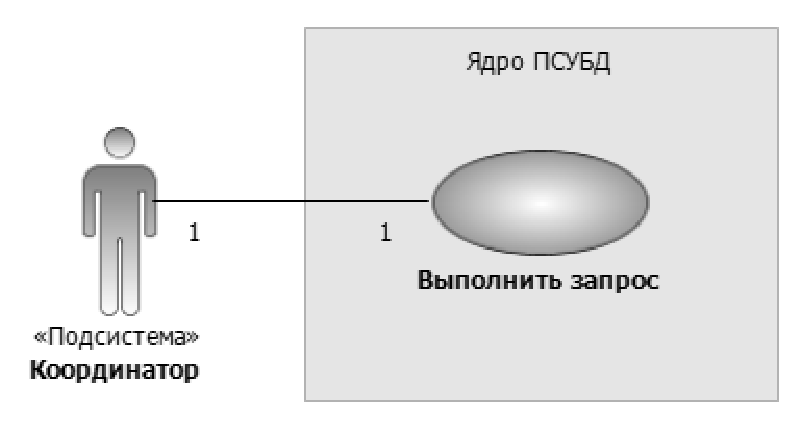
\includegraphics[width=0.7\linewidth]{kernelUCDiagram}
		\caption{}
		\label{fig:kernelucdiagram}
	\end{figure}
	
	
	Для подсистемы "<Ядро ПСУБД"> нами был разработан вариант использования \textit{"<Выполнить запрос">}, приведенный на рис. ~\ref{fig:kernelucdiagram}.
	. Варианты использования Ядра ПСУБД спроектированы с расчетом на дальнейшее расширение функциональности данной подсистемы. Далее в этом разделе приводится детальное описание варианта использования.
	
	\subsubsection{Вариант использования "<Выполнить запрос">}
	\par Выполняет обработку запроса. Вариант использования начинается, когда Координатор вызывает функцию "<Выполнить запрос">.
	\par Основной поток событий состоит из следующей последовательности шагов. На первом шаге Ядро ПСУБД получает от Координатора запрос в виде текстового файла в асинхронном режиме. На втором шаге Ядро ПСУБД выполняет разбор запроса, строит дерево запроса, формирует последовательный физический план запроса. На третьем шаге строится параллельный план путем добавления оператора \texttt{Exchange} в дерево запроса. На третьем шаге Ядро ПСУБД запускает параллельный план в виде параллельного агента (независимого системного процесса), который начинает обработку запроса в асинхронном режиме. Согласованную работу агентов на различных узлах обеспечивает оператор \texttt{Exchange}. На четвертом шаге параллельный агент выполняет обработку запроса. По завершении обработки Ядро ПСУБД сохраняет результат в результирующий файл и код возврата, полученный от параллельного агента, в лог-файл.
	На последнем, пятом шаге, Ядро ПСУБД передает Координатору лог-файл и результирующий файл. Вариант использования завершается.
	
	\section{Заключение}\label{S_Conclusion}
	\par В данной работе представлены спецификации параллельной системы управления базами данных для грид-систем. Спецификации описаны при помощи модели вариантов использования с использованием языка моделирования UML. Описана общая схема обработки запросов в такой ПСУБД.
	\par В качестве направлений дальнейшей работы можно выделить следующие. Во первых, планируется разработка модели проектирования ПСУБД, учитывающей такие особенности грид-систем как неоднородность вычислительных узлов и неоднородность соединительной сети. Во-вторых, мы предполагаем реализовать описанные в модели вариантов использования спецификации в прототипе ПСУБД.
	\par{\it Работа выполнена при финансовой поддержке Российского фонда фундаментальных исследований (проект 06-07-89148).}
	% оформление библиографии
	\begin{thebibliography}{X}
		\bibitem{B_Gray2005} {\bf Gray J.} {\sf Query Evaluation Techniques for Large Databases} / J. Gray // ACM Computing Surveys.--1993. --Vol. 25 №{2} --P. 73--169\vspace{-2mm}
		
		\bibitem{B_Mehta1997} {\bf Mehta M.} {\sf Data Placement in Shared-Nothing Parallel Database Systems} / M. Mehta, D.J. DeWitt // The VLDB Journal. --1997. --Vol. 6 №{1} --P. 53--72\vspace{-2mm}
		
		\bibitem{B_Williams1998} {\bf Williams M.H.} {\sf Data Placement in Parallel Database Systems} / M.H. Williams, S. Zhou // Parallel Database Techniques. --1998. --P. 203--218\vspace{-2mm}
		
		\bibitem{B_OMEGA} {\bf Проект "<Омега">.} {\sf  Разработка параллельной СУБД для мультипроцессорных вычислительных систем с кластерной архитектурой}\ (http://omega.susu.ru/).
		
		%\bibitem{B_Sokolinsky2004} {\bf Соколинский Л.Б.} {\sf Обзор архитектур параллельных систем баз данных} / Л.Б. Соколинский // Программирование. --2004. №{6} --С. 49--63\vspace{-2mm}
		
		\bibitem{B_Sokolinsky2001} {\bf Соколинский Л.Б.} {\sf Организация параллельного выполнения запросов в многопроцессорной машине баз данных с иерархической архитектурой} / Л.Б. Соколинский // Программирование. --2001. №{6} --С. 13--29\vspace{-2mm}
		
		\bibitem{B_Aloisio2005} {\bf Aloisio G.} {\sf The Grid-DBMS: Towards Dynamic Data Management in Grid Environments} / G. Aloisio, M. Cafaro, S. Fiore, M. Mirto // Proceedings of the International Conference on Information Technology: Coding and Computing (ITCC'05). --2005. --Vol. 2 --P. 199--204\vspace{-2mm}
		
		\bibitem{B_Dutra2004} {\bf Dutra M.L.} {\sf An adaptive parallel query processing middleware for the grid} / DaSilva V.F., Dutra M.L., Porto F., Schulze B., Barbosa A. C., de Oliveira J.C. // Concurr. Comput. : Pract. Exper. --2006. --Vol. 18 №{6} --P. 621--634\vspace{-2mm}
		
		\bibitem{B_Lepikhov2006} {\bf Лепихов А.В.} {\sf Стратегия размещения данных в многопроцессорных системах с симметричной иерархической архитектурой} / Лепихов А.В., Соколинский Л.Б. // Научный сервис в сети Интернет: технологии параллельного программирования: Труды Всероссийск. науч. конф. (18-23 сентября 2006 г., г. Новороссийск). --М: Издательство МГУ, --С. 39--42\vspace{-2mm}
		
		%\bibitem{B_TechReport13_2007} {\bf Лепихов А.В.} {\sf Модель вариантов использования параллельной  системы баз данных "<Омега">} / А.В. Лепихов, Л.Б. Соколинский // Технич. отчет OMEGA13. --Челябинск: ЮУрГУ, 2007. --15 с.\vspace{-2mm}
		
		%\bibitem{B_TechReport16_2008} {\bf Лепихов А.В.} {\sf Модель проектирования параллельной  системы баз данных "<Омега">} / А.В. Лепихов, Л.Б. Соколинский // Технич. отчет OMEGA16.--Челябинск: ЮУрГУ, 2008. --~20~с.\vspace{-2mm}
		
		\bibitem{B_RFC4180} {\bf RFC4180:} {\sf Common Format and MIME Type for Comma-Separated Values (CSV) Files:}\\ (http://tools.ietf.org/html/rfc4180), October 2005. \vspace{-2mm}
		
	\end{thebibliography}
	
	
\end{document}